
\section{Application to state price densities implied from option prices}\label{t4}

In this section we analyses the state price densities (SPD) implied by the stock index option prices. As state dependent contingent claims, they contain information about the risk factors driving the underlying asset price process and give information about expectations and risk patterns on the market. Mathematically, SPDs are equivalent martingale measures for the stock index and their existence is guaranteed in the absence of arbitrage plus some technical conditions. A very restrictive model, with log-normal marginals for the asset price, is the Black-Scholes model. This model results in log-normal SPDs that correspond to a constant implied volatility surface across strikes and maturity. This feature is inconsistent with the empirically documented volatility smile or skew and the term structure. Therefore, richer specifications for the option dynamics have to be used. Most of earlier works adopt a static viewpoint; they estimate curves separately at different moments in time, see the methodology reviews by \cite{Bahra1997}, \cite{Jackwerth:99} and \cite{Bliss2002}. In order to exploit the information content from all data available, it is reasonable to consider them as collection of curves. 

The relation between the SPDs and the European call prices has been demonstrated by \cite{Breeden:78} and \cite{Banz:78} for a continuum of strike prices spanning the possible range of future realizations of the underlying asset. For a fixed maturity, the SPD is proportional to the second derivative of the European call options with respect to the strike price. In this case, SPDs are one-dimensional functions. A two-dimensional point of view can be adopted if maturities are taken as an additional argument and the SPDs are viewed as a family of curves.

%From a statistical perspective, SPD is intrinsically related to the data generation process of the underlying stock index. Mathematically, it is an equivalent martingale measure for the stock index, whose existence is guaranteed in the absence of arbitrage plus some technical conditions  A very restrictive model, with normal marginal distributions, is the Black-Scholes model. This model results in log-normal densities for SPDs. They correspond to a constant implied volatility surface across strikes and maturity, a feature that is inconsistent with the empirically documented volatility smile or skew and the term structure. Therefore, richer specifications for the option dynamics have to be used. 

%have been proposed, e.g., \cite{Bates:96}, \cite{Pan:02}, \cite{Chernov:03} and \cite{Eraker:03}. They include local volatility function, a stochastic diffusion coefficient, jump intensities, jump amplitudes etc. However, they still fail to reproduce the features embedded in the option returns, see \cite{Bakshi:97}, \cite{Bates:00} and \cite{Eraker:04} for instance. As \cite{Cont:02} observe, the options markets have become increasingly autonomous include specific sources of randomness not present in the underlying's dynamics.   

%A lot of work has been done use calls/puts equivalent IV surfaces \cite{Bakshi:00}. We will return to this point at a later point in section ?. 

%Nonparametric estimation of SPDs from option prices has been pioneered by \cite{Jackwerth:96}, \cite{Sahalia:98}, \cite{Jackwerth:00}. The monograph by \cite{Jackwerth:99} provides an excellent and comprehensive review of the literature on this topic, covering both methodological issues and applications.  \cite{Bliss2002} give as well a very good overview of the alternative approaches for extracting SPDs, as well as the problems associated with different methods. \cite{Bahra1997} is another often-cited methodology review. 

%Most of earlier works adopt a static viewpoint; they estimate curves separately at different moments in time. In order to exploit the information content from all data available, it is reasonable to consider them as collection of curves. %An important methodological contribution in this field pertains to the FPCA, which allows explaining complicated data structures with a few components. In addition, the principal scores can be used to study the variation of the observed phenomena. In this paper we aim to close the existent theoretical gap in the literature on FPCA for the study of derivatives of functions in high-dimensions and to apply the newly developed framework to the study of SPDs.


%Our empirical study is motivated by the evolution of state price densities (SPD) implied by option data. 
%Option prices, as state dependent contingent claims, contain information about the risk factors driving the underlying asset price process and give information about expectations and risk patterns on the market. %In a discrete Arrow-Debreu setup, if there is an equal number of states and state-dependent contingent claims, then the price of any asset can be derived as a weighted average of the state prices. The SPD is the continuous counterpart of the Arrow-Debreu prices. Its link to European option prices has been demonstrated by \cite{Breeden:78} and \cite{Banz:78}, for a continuum of strike prices spanning the possible range of future realizations of the underlying.

%For a fixed maturity and under some general arbitrage conditions the SPD is proportional with the quotient of the European call options with respect to the strike price. If only options with a pre-specified maturity are to be analyzed, then SPDs are one-dimensional functions. A two-dimensional point of view can be adopted if maturities are taken as an additional argument and the SPDs are viewed as a family of curves.
Let $C: \mathbb{R}_{\geq 0}^{2}\rightarrow \mathbb{R}$ denote the price function of a European call option with strike price $k$ and maturity $\tau$ such that
%In an arbitrage-free market, the price $C$ of a European call is obtained by discounting the expected payoff, where the expectation is taken with respect to the state price measure
\begin{equation}\label{c:c2}
C(k,\tau) = \exp{(-r_{\tau}\tau)}\int_0^\infty(s_{\tau}-k)^{+} q(s_{\tau},\tau) \,ds_{\tau},
\end{equation}
where $r_{\tau}$ is the annualized risk free interest rate for maturity $\tau$, $s_{\tau}$ the unknown price of the underlying asset at maturity, $k$ the strike price and $q$ the state price density of $s_{\tau}$. % $\tau$ the time to maturity  %, $s_{\tau}$ denotes all possible realizations of the random variable $S_{\tau}$ and  $q(s_{\tau},\tau |r_{\tau}, s_0)$ is the conditional risk neutral density. 
%For fixed $r_{\tau}$ and $s_0$ within one day we write $q(s_{\tau},\tau)$ and $C(k,\tau)$ for the respective quantities in (\ref{c:c2}) to keep notation simple. The proportionality relationship between the SPD and the second derivative of the call price with respect to the strike price can then be written as: 
One can show that 
 \begin{equation}\label{q09}
    q(s_{\tau},\tau) =\exp{(r_{\tau}\tau)}\left. \frac{\partial^2 C(k,\tau)}{\partial k^2} \right|_{k=s_{\tau}}.
\end{equation}
Let $s_0$ be the asset price at the moment of pricing and assume it to be fixed. Then $F=\exp(r_{\tau}\tau)s_0$ is called the forward price. Suppose that the call price is homogeneous of degree one in the strike price. Then it holds that
\begin{equation}\label{q10}
C( k,\tau) = F C(k/F,\tau).
\end{equation}
%as it the case of the Black-Scholes model, 
%for any constant $s_0$. 
If we denote $m=k/F$ the moneyness, it is easy to verify that 

\begin{equation}\label{q}
\frac{\partial^2 C(k,\tau)}{\partial k^2}=\frac{1}{F}\frac{\partial^2 C(m,\tau)}{\partial m^2}.
\end{equation}
Using our previous notations, in our application $X(t)$ will refer to $C(m,\tau)/F$ and its second derivative with respect to the moneyness, $X^{(2,0)}$ will specify the density of future returns $q(s_{\tau}/s_0,\tau)=s_0q(s_{\tau},\tau)$. %The underlying assumption is that the conditional distribution of returns is stationary. 
In practice, when analyzing a sample of curves, it is preferable to work with densities of future assets returns rather than prices because the underlying functions become location invariant. %rather than prices because prices are often non-stationary, which causes that the salient features of the functions do not occur at the same location in the argument's space.  %be shifted on the same support. are assumed to be stationary. This insures that realizations of SPD share the same domain. %There is a practical argument for proceeding in this way when applying FPCA: \textit{Reformulate: the variability of the observed domain of $X$ over time is large and without standardization the common support of the observable in this dimension is very small. If conditional distribution of returns is stationary this should insure that SPD functions sharing the same space over time (why? reference).} %In addition, the results seem to be more

%From a statistical perspective, state price density is intrinsically related to the data generation process. A very restrictive model, with normal marginal distributions, is the Black-Scholes model. The application of this model results in a log-normal state price. This is equivalent to a constant volatility across strikes, a feature that is inconsistent with the empirically documented volatility smile of skew. Therefore, richer parametric specifications or nonparametric models have been accounted for to estimated SPDs from the option data. 

%Nonparametric estimation of SPD has been pioneered by from option prices \cite{Jackwerth:96, Sahalia:98, Jackwerth:00}.  Many of the differences are based on the nonparametric smoothing techniques. The monograph by \cite{Jackwerth:99} provides an excellent and comprehensive review of the literature on this topic, covering both methodological issues and applications.  \cite{Bliss2002} also give a very good review of the alternative approaches to extracting the RND and the problems that arise with different methods. \cite{Bahra1997} is another often-cited review of methodology.

%Most of earlier works adopt a static viewpoint; they estimate curves separately at different moments in time. In order to exploit the information content of all this data it is reasonable to consider them as collection of curves. We will assume that the stock price index is a semimartingale. Within one trading day $i$ options written on the same underlying are traded for different expiration dates and various moneyness. 

%Let $C_i: \mathbb{R}^{2}\rightarrow \mathbb{R}$ be a smooth response call price function on day $i$, for $t=(m,\tau)$. We denote by $Y_i=C_i-\EE\left[C\right]$ the demeaned functions and assume the model ($\ref{basic}$) for the centered observed call prices $X_i(t_{ik})$. %The state variables $(s_{i0},r_{i\tau })$ are implicitly embedded in $C_i$. 

%For observations $Y_{i}$ at discrete $t_i$, for $i=1, \ldots , N$, we assume that the following model holds
%\begin{equation}\label{z}
%X^C_{i}(t_i)\stackrel{\operatorname{def}}{=} C_i(t_{j})+\varepsilon_{ij}, \quad i=1, ... , n
%\end{equation}
%where $C_i: \mathbb{R}^{2}\rightarrow \mathbb{R}$ are smooth functions in both dimensions and $\varepsilon_{ij}$ has $\mathsf{E}[\varepsilon|\textbf{t}_i]=0 $ and $\mathsf{Var}[\varepsilon|\textbf{t}_i]=\sigma_i^2 $. The state variables $(s_{0i},r^f_{\tau i})$ are implicitly embedded in $C_i$.

%Following the steps explained in section \ref{noise} we obtain estimates of the SPDs:
%For $d=(2,0)$ we obtain estimates of the SPDs:
%\[
%\hat{q}_{i,PCA}(\textbf{t}_i)= \sum_{r^*=1}^{L}  \hat{\delta}_{ir^*;T} \hat{\gamma}^q_{r^*;T}(\textbf{t}_i),
%\]
%\[
%\hat{\gamma}^q_{r,T}(\textbf{t}_i)= \frac{1}{\sqrt{\hat{l}_{r}}} \sum_{j=1}^N \hat{p}_{rj} \hat{q}_{i,h}(\textbf{t}_i),
%\]
%\begin{equation*}
%\hat{q}_{i,FPCA}(r_{s,\tau},\tau)=e^{r_{i\tau}\tau}\hat{C}^{(2,0)}_{i,FPCA} (m,\tau)\big|_{m = r_{s,\tau}}.
%\end{equation*}
%$\hat{\delta}$, $\hat{l}$ and $\hat{p}$ the loadings, eigenvalues and eigenvectors computed by applying the spectral decomposition on $\hat{M}$; $\hat{q}_{i,h}$ a smooth estimate of the RND on day $i$ as explained in subsection \ref{locpol} with $\hat{C}^{(2)}_i$ the local polynomial estimate for the second derivative of the call price function $C_i$ with respect to the moneyness $m$.


\subsection{Implementation}\label{implementation}

\subsubsection{Centering the observed curves } %Estimation of $\hat{M}^{(\nu)}$ }
%In our case $p=3, d_K=2, d_\tau=0, g=2$. The observed call prices are not centered, therefore we center observations.
Throughout the paper it is assumed that the curves are centered. To insure this assumption, we subtract the empirical mean $\bar{X}^{(\nu)}(t_k) = \frac{1}{N} \sum_{i=1}^{N} \hat{X}^{(\nu)}_{i,b}(t_k)$ from the the observed call prices to obtained centered curves. A centered version $\overline{M}^{(\nu)}, \; \nu=(0,d)$ is given by 
\begin{equation}
\label{demean}
\overline{M}^{(\nu)}_{ij} = \hat{M}^{(\nu)}_{ij} - \frac{1}{T} \sum_{k=1}^T\left(  \bar{X}^{(\nu)}(t_k) \hat{X}^{(\nu)}_{i,b}(t_k) +  \bar{X}^{(\nu)}(t_k) \hat{X}^{(\nu)}_{j,b}(t_k) - \bar{X}^{(\nu)}(t_k)^2 \right).
\end{equation}
There is still space for improvement when centering of the curves. One possibility is to use a different bandwidth to compute the mean because averaging will necessarily lower the variance. Secondly, by the arguments of Section \ref{intest}, the $\frac{1}{T} \sum_{k=1}^T \bar{X}^{(\nu)}(t_k)^2$ term can be improved accordingly to Lemma \ref{lemint} by subtracting $\hat{\sigma}_\varepsilon$ weighted by suitable parameters. We decide to omit these fine tunings in our application because it would involve a huge amount of additional computational effort in contrast to only minor improvements in the results. 


\subsubsection{Bandwidth selection}

To get  rates of convergence for $\hat{M}^{(d)}$ related  to Remark \ref{remark1} we choose $\rho=7$ and $b$ has to lie between $\mathcal{O}(T^{-1/10})$ and $\mathcal{O}(T^{-1/12} )$. 
The choice of $b$ to estimate $\hat{M}^{(0)}$  is similar, with the difference that $\rho>0$, we choose $\rho=1$ and $b$ has to lie between $\mathcal{O}(T^{-1/3})$ and $\mathcal{O}(T^{-1/5} )$.
We use a very easy criteria to choose the bandwidth because by Proposition \ref{asymgam} the dominating error depends mainly on the choice of $h$.
Let $t_{ik}=(t_{ik1}, \dots t_{ikg})$, then the bandwidth for direction $j$ is determined by $b_{j} = \left( (\max_k(t_{ikj})- \min_k(t_{ikj})  )T_i \right)^\alpha$. When estimating state price densities $t_{ik}=(\tau_{ik},m_{ik})$ and $T_i$ is replaced by the cardinality of $\tau_{i}=\{\tau_{i1},\dots \tau_{i T_i}\}$ and $m_{i}$ respectively. 
%and we determine the bandwidth with $b_{i \tau} = \left((\max(\tau_{i})- \min(\tau_{i})) |\tau_{i}| \right)^\alpha$ for the maturity direction where $|\tau_{i}|$ is the cardinality of the set $\tau_{i}=\{\tau_{i1},\dots \tau_{i T_i}\} $. 
%The bandwidth for the moneyness direction is chosen likewise. 
 In the estimation of $\hat{M}^{(d)}$ we set $\alpha=-1/10$ and $\alpha=-1/3$ for $\hat{M}^{(0)}$. %We correct the individual bandwidth for the order of the optimal bandwidth and thus use $b_j= (N^{-1} \sum_{i=1}^N h_{ij,ind})^{10/3}$. %based on the individual optimal bandwidths and adjust for the smallest allowed bandwidth..% and adjust for the smallest allowed bandwidth.

% and analogously the empirical mean of the presmoothed curves to compute $\hat{M}^{(d)}$ .
%\[
%X_i(t)\stackrel{\operatorname{def}}{=}   X^C_i(t) - N^{-1} \sum_{i=1}^N X^C_i(t).
%\]
%For $d=(2,0)$, to estimate $M^{(d)}$ we center smoothed estimates of call surface %with bandwidth $b$ 
%\[
%\hat{Y}^{(d)}_{b,i}(t)\stackrel{\operatorname{def}}{=}   \hat{C}^{(d)}_{b,i}(t) - N^{-1} \sum_{i=1}^N \hat{C}^{(d)}_{b,i}(t) .
%\]

\label{operbw}
The choice of bandwidths $h$ is a crucial parameter for the quality of the estimators. %, while the choice of $b$ is negligible under certain conditions. 
%For the numerical study 
%We use as guidance the optimal multivariate theoretical bandwidth from Section \ref{estderiv}. % and adapt the approaches of \cite{Fan:96} or \cite{Yang:15} to our setup. 
To derive an estimator for the bandwidths first note that in the univariate case $(g=1)$
 %The optimal bandwidth for the individual curves, as well as the optimal bandwidth choice $b$ to estimate $M^{(d)}$ are of the same order. %Therefore, we will use the obtained bandwidth in both cases. 
%Possible solutions for the choice of $h$ include cross-validation, as suggested by \cite{Benko:2009} or operationalization of the optimal multivariate theoretical bandwidth in section \ref{t3} by adapting the approaches of \cite{Fan:96} or \cite{Yang:15} to our setup. Considering  the computational effort needed to implement these, we decided to follow a simpler path. To obtain the optimal bandwidths, we treat every dimension as if we have to choose an optimal bandwidth for the univariate case and correct for the asymptotic order. %The optimal bandwidth for the individual curves, as well as the optimal bandwidth choice $b$ to estimate $M^{(d)}$ are of the same order. %Therefore, we will use the obtained bandwidth in both cases. 
the theoretical optimal univariate asymptotic bandwidth for the $r$-th basis is given by 
\begin{equation}\label{opt}
h^{d,\nu}_{r,opt} = C_{d,p}(K) \left[T^{-1}\frac{ \int_0^1 \sum_{i=1}^N (p^{(\nu)}_{ir})^2 \sigma_{\varepsilon i} ^2 (t) f_i(t)^{-1} dt}{ \int_0^1 \left\{ \sum_{i=1}^N p^{(\nu)}_{ir} X_i^{(p+1)} (t)    \right\}^2 dt} \right]^{1/(2p+3)} , %\; t_1=m, t_2=\tau
\end{equation}
\[
C_{d,p}(K)=\left[ \frac{(p+1)!^2(2d+1) \int K^{*2}_{p,d_j}(t)dt }{2(p+1-d) \{\int u^{p+1} K_{d,p}^*(t)dt \}^2}\right]^{1/(2p+3)}.
\]
Like in the conventional local polynomial smoothing case $C_{d,p}(K)$ does not depend on the curves and is an easily computable constant. It only depends on the chosen kernel, the order of the derivative and the order of the polynomial, see for instance \cite{Fan:96}. %To derive the individual bandwidth for a single curve $X_i$, we have to set $p^{(\nu)}_{ir}=1$ while  $p^{(\nu)}_{jr}=0 \; \forall i\neq j$.

For our bandwidth estimator we treat every dimension separately, as if we have to choose an optimal bandwidth for derivatives in the univariate case, and correct for the asymptotic order, see Section \ref{estderiv}.
In practice, we can not use equation (\ref{opt}) to determine the optimal bandwidth because some variables are unknown and only discrete points are observed.  As a rule-of-thumb, we replace these unknown variables using approximations. 
Estimates of $p^{(0)}_{ir}$ from $\hat{M}^{(0)}$ and $p^{(d)}_{ir}$ from $\hat{M}^{(d)}$ are further used. With these approximations, a feasible rule for computing the optimal bandwidth in direction $j$ for the $r$-th basis function $h_{jr}$ is given by
\begin{equation}\label{rulethumb}
h^{d,\nu}_{jr,rot} =\left(  T^{-1} \frac{C_{d,p}^{2p+3}\hat{\sigma}^2_{\varepsilon}  } { f_j \int_0^1 \left\{ \sum_{i=1}^N \hat{p}^{(\nu)}_{ir} \tilde{X}_i^{(p+1)} (t_j)    \right\}^2 d t_j } \right)^{1/(g+2p+2)}.
%h^{(\nu)}_{jr,rot} =\left(  T^{-1} \frac{C_{d,p}^{2p+3}\hat{\sigma}^2_{\varepsilon} \int_0^1 \hat{f}_{t_j}(t_j)^{-1}dt_j } {  \int_0^1 \left\{ \sum_{i=1}^N \hat{p}^{(\nu)}_{ir} \tilde{X}_i^{(p+1)} (t_j)    \right\}^2 d t_j } \right)^{1/(g+2p+2)}.
%h_{rot}\left\{ \bullet \right\} = C_{d,p} \left( T^{-1} \frac{\hat{\sigma}_{\epsilon} } {  \int_{[0,1]^g} \left\{ \sum_{j=1}^N \hat{p}^{(\nu)}_{jr} \hat{Y}_j^{(p+1)} (t)    \right\}^2 dt } \right)^{1/(g+2p+3)} 
%h_{s,rot}\left\{ \bullet \right\} = C_{d,p} \left( \left(T^{-1}\sum_{i=1}^T \right) \frac{\hat{\sigma}_{\epsilon} } {  \int_0^1 \left\{ \sum_{j=1}^N \hat{p}^{(\nu)}_{jr} Y_j^{(p+1)} (t)    \right\}^2 dt } \right)^{1/(2p+3)} 
\end{equation}
%$\hat{\sigma}^2_{\varepsilon}$ is estimated as described in section \ref{estsig}. 
In our application as well as our simulation we have $g=2$, $d=(0,2)$ and do a third order local polynomial regression. The integrals are approximated by Riemann sums. 

\begin{itemize}
	\item The density of the observed points is approximated by a uniform distribution with $f_1= \max_{i,j}(\tau_{ij})- \min_{i,j}(\tau_{ij})$ and $f_2= \max_{i,j}(m_{ij})- \min_{i,j}(m_{ij})$.
	
		\item To get a rough estimator for $ X_i^{(p+1)}$ based on $X_i$, we use a polynomial regression.  % as recommend by \cite{Fan:96}. %For $\nu=0$ we can alternatively perform a local polynomial regression at $ \sum_{j=1}^N \hat{p}_{jr} \hat{Y}_j^{(p+1)_i} (u_i) = \hat{\gamma}^{(p+1)_i}(u_i)$ which might give better results. 
%The estimate for $Y^{(p+1)_{u_i}}$ using polynomial regression is given by
For our application, we take $p=3$ and are thus interested in estimates for $X_i^{(4)}(m)$ and $X_i^{(4)}(\tau)$. We expect the curves to be more complex in the moneyness direction than in the maturity direction and we adjust the degree of the polynomials to reflect this issue. The estimates are then given by% In general it is not necessary to use the same $p$ for the estimation of $M^{(d)}$ and $Y^{(d)}$, but because the required $p$ to get the desired convergence rates for $M^{(d)}$ is still considerably small we use $p=5$ for both estimations. 
\begin{equation}
\begin{split}
%a^*_i=&\operatorname{arg}\,\underset{a_i}{\operatorname{min}} \left( X_i(m,\tau) - a_{i0} + \sum_{l=1}^5 a_{il} m^l + \sum_{l=6}^{10} a_{il} \tau^{(l-5)} \right) \\
a^*_i=&\operatorname{arg}\,\underset{a_i}{\operatorname{min}} \left( X_i(m,\tau) - a_{i0} + \sum_{l=1}^5 a_{il} m^l + \sum_{l=6}^{9} a_{il} \tau^{(l-5)} \right) \\
\tilde{X}_i^{(4)}(m)  = & 24 a^*_{i4} + 120 a^*_{i5} m  \\%6 a^*_{i3}+ 24 a^*_{i4} m + 120 a^*_{i5} m^2  \\
%\tilde{Y}_i^{(4)}(\tau) & = 24 a^*_{i9} + 120 a^*_{i10} \tau %6 a^*_{i8}+ 24 a^*_{i9} \tau \\
 \tilde{X}_i^{(4)}(\tau)  = & 24 a^*_{i9}.  %6 a^*_{i8}+ 24 a^*_{i9} \tau \\
 \end{split}
\end{equation}
		
			\item \label{estsig}
To estimate the variance for each curve we use the kernel approach given in (\ref{varestim}) using a Epanechnikov kernel with a bandwidth of $T^{-2/(4+g)}$ for each spatial direction. These estimates are used as well to correct for the diagonal bias when $\hat{M}^{(0)}$ and $\hat{M}^{(d)}$ are estimated. In (\ref{rulethumb}) the average over all $\hat{\sigma}_{i,\epsilon}$ is used. %In the simulation study we estimate the variance once and use the estimated values for each of the methods.  %We can derive a very rough estimate by setting $h_{i,0}=(NT)^{-1/(2p+3)}$
%Because $g=2$, a difference based estimator for $\sigma_{\epsilon,i}$ is used, to make the computation easier we additionally assume that $f\in C^{(2)}[0,1]^2$ here. Let $m$ be ordered and $\Delta=\frac{1}{\sqrt{1.5}} (- 0.5,1 ,- 0.5)$. Let further $\tilde{T}_{il}$ be the number of observations for curve $i$ with maturity $\tau_l, \; l=1,\dots,M$ then
%\begin{equation}
%%\hat{\sigma}^2_{\epsilon,i}= \frac{1}{5*48} \sum_{l=1}^5 \sum_{j=2}^{49} \left( \sum_{k=1}^3 \Delta_k C_i(K_{i(j-2+k)l},\tau_l) \right)^2
%\hat{\sigma}^2_{\varepsilon,i}= \frac{1}{\left(\sum_{l=1}^M \tilde{T}_{il}-2 \right)} \sum_{l=1}^M \sum_{j=2}^{\tilde{T}_{il}-1} \left( \sum_{k=1}^3 \Delta_k Y_i(m_{i(j-2+k)l},\tau_l) \right)^2.
%\end{equation}
%For the application we assume that $\sigma_{\varepsilon}=\sigma_{\varepsilon,i} \; \forall i$. Therefore the empirical mean $\hat{\sigma}^2_{\varepsilon}= N ^{-1}\sum_{i=1}^N \hat{\sigma}^2_{\varepsilon,i}$ is used for further computations. This estimate is used as well to correct for the diagonal bias if $\hat{M}^{(0)}$ and $\hat{M}^{(d)}$ are estimated. %We can derive a very rough estimate by setting $h_{i,0}=(NT)^{-1/(2p+3)}$

\end{itemize}

For technical reasons, we use the product of Gaussian kernel functions to construct local polynomial estimators. The reason for is that, as we can verify from Proposition \ref{hhvar}, the optimal bandwidth $h$ will decrease in $N$. By using a global bandwidth and a compact kernel the matrix given in equation (\ref{STMat}) may become singular when $N$ is large and $T$ is small. 

% 
 In our simulation and application we use the mean optimal $h^{d,\nu}_{i,rot}= L^{-1} \sum_{r=1}^L h^{d,\nu}_{ir,rot} $ for each $\hat{\gamma}^{(d)}_r, \hat{\varphi}^{(d)}_r$ to save computation time. %An estimator for the individual optimal bandwidth $h_{ij,ind}$ of each curve $i$ is obtained by replacing $\sum_{i=1}^N \hat{p}^{(\nu)}_{ir} \tilde{Y}_i^{(p+1)}(t_j)$ with $\tilde{Y}_i^{(p+1)}(t_j)$.
Since we had to demean the sample in (\ref{demean}), finally we add  $N^{-1} \sum_{i=1}^N \hat{X}^{(d)}_{i,h^{d,\nu}_{i,rot}}$ to the resulting truncated decomposition to derive the final estimate.



\subsubsection{Estimation of the number of components}
In Section \ref{Lchoi} we assumed that the number of components is given. In general, the number of basis functions needed is unknown a priori. For the case $max(d)=0$ there exists a wide range of criteria that can be adapted to our case to determine the upper bound $L$. The easiest way to determine the number of components is by choosing the model accuracy by an amount of variance explained by the eigenvalues. %Usual values are 80$\%$, 90$\%$ or 95$\%$.  
In (\ref{lambdabias}) we show that under the conditions from Proposition \ref{asymgam} $\hat{\lambda}^{(d)}_r-\hat{\lambda}_{r;T}^{(d)} = \mathcal{O}_p(N^{-1/2}T^{-1/2} + T^{-1})$ and $\lambda^{(d)}_r-\hat{\lambda}_{r}^{(d)} = \mathcal{O}_p(N^{-1/2})$. The assumptions in Corollary 1 from \cite{Bai2002} can be adapted to our case and give several criteria for finding $L$ or $L_d$ by generalizing \cite{Mallows:73} $C_p$ criteria for panel data settings. % by using $\hat{\lambda}^{(d)}_{r;T}, \; d=0,d$ in (\ref{optk}).
These criteria imply minimizing the sum of squared residuals when $k$ factors are estimated and penalizing the overfitting. 
One such formulation suggests choosing the number of factors using the criteria% which for some constant $C_{NT}=\min(\sqrt{N},\sqrt{T})$ and a prespecified $L^{\max}< \min(N,T)$ given by %and a consistent estimator $\hat{\sigma}_{\varepsilon}$ for $N^{-1} \sum_{i=1}^N \sigma_{\varepsilon,i}$ the optimal $K$
%fulfilled and to the problem is given a criteria from \cite{Bai2002}.
\begin{equation}\label{optk}
%K= \operatorname{arg}\,\underset{k\in \mathbb{N}}{\ope-ratorname{min}}  \left[ \log\left(\sum_{r=k+1}^N \hat{\lambda}_r\right)  + k\left( \frac{N+T}{NT} \right) \log\left(\min(N,T) \right) \right]
%K= \operatorname{arg}\,\underset{k\in \mathbb{N}}{\operatorname{min}}  \left[ \log\left(\sum_{r=k+1}^N \hat{\lambda}_r\right)  + k\left( \frac{log(C^2_{NT})}{C^2_{NT}} \right)  \right].
%\operatorname{arg}\,
PC^{(\nu)}(k^*)=\underset{k\in \mathbb{N}, k\leq L_{\max}}{\operatorname{min}}  \left[ \left(\sum_{r=k+1}^N \hat{\lambda}^{(\nu)}_{r}\right)  + k \left(\sum_{r=L^{\max}}^N \hat{\lambda}^{(\nu)}_{r}\right)  \left( \frac{\log(C^2_{NT})}{C^2_{NT}} \right)  \right],
\end{equation}
for the constant $C_{NT}=\min(\sqrt{N},\sqrt{T})$ and a prespecified $L^{\max}< \min(N,T)$. Alternatively, \cite{Bai2002} propose an information criteria that do not depend on the choice of $L_{\max}$. We consider the above modified criteria
\begin{equation}\label{optIC}
IC^{(\nu)}(k^*)=\underset{k\in \mathbb{N}, k\leq L_{\max}}{\operatorname{min}}  \left[ \log {\left(\frac{1}{N}\sum_{r=k+1}^N \hat{\lambda}^{(\nu)}_{r}\right)}  + k  \left( \frac{\log(C^2_{NT})}{C^2_{NT}} \right)  \right].
\end{equation}
Here using $\nu=(0,\dots,0)^\top$ will give $L$ while using $\nu=d$ will give the factors $L_d$.

Another possibility for the choice of number of components is to compute the variance explained by each nonorthogonal basis by 
\begin{equation}\label{varnno}
\var(\hat{\delta}_{r,T}^{(d)}\hat{\gamma}_{r,T}^{(d)})=\langle \hat{\gamma}_{r,T}^{(d)},\hat{\gamma}_{r,T}^{(d)}\rangle\hat{\lambda}_r,
\end{equation}
%This provides an estimate of the upper bound $L$ for $|d|=0$ and of the number of eigenfunctions $L_d$ for the decomposition of derivatives for $|d|>0$ in (\ref{approx12}).
order them and use equations \eqref{optk} or \eqref{optIC} to select the number of components.
%\color{red} %To derive the results of Proposition (\ref{Mbias}) and (\ref{asymgam}) it is not necessary that to require that $X$ has a factor model structure. 
%Estimating derivatives or high-dimensional spatial curves with high accuracy is a difficult task as we can verify by the rates for the individual curves given by  (\ref{bias_var}). Under the factor model assumption however it is possible to improve even for the estimation of individual curves the rate of convergence using our methods. In general our estimates are better than using local polynomial estimators for each curve individually, because equation (\ref{naiveev}) and (\ref{evd}) can be interpreted as an average over $N$ curves for only a finite number of $L$ components.  The intuition behind is, that only  components are truncated which are related to the error term and thus a more accurate fit is possible. \color{black}



\subsection{Simulation Study}\label{simstudy}


%\subsection{Generating Noisy Curves}
We investigate the finite sample behavior of our estimators in a simulation study, which is guided by the real data application in Section \ref{realData}. 
%We consider mixtures of $L+1$ $\log\mathcal{N}(\mu_l, \sigma_l)$ density functions with mixture weights $w_{il}$ where $i$ is the day, $ l=1,\ldots,L+1$ and $\sum_{l=1}^{L+1} w_{il}=1 $. Then the true SPDs are given by:
Simulated SPDs are modeled as mixtures of $L$ components, $q(m,\tau)=\sum_{l=1}^{L}w_lq^l(m,\tau)$, where $q^l$ are fixed basis functions and $w_l$ are random weights. For fixed $\tau$ we consider $q^l(\cdot,\tau)$ to be a log-normal density functions, with mean $\left(\mu_l-\frac{1}{2}\sigma_l^2\right)\tau$ and variance $\sigma_l^2 \tau$, and simulate weights $w_{il}$ with $\sum_{l=1}^{L} w_{il}=1 $, where $i=1,\ldots,N$ is the index for the day, then %The SPDs are thus given by:
\begin{equation}
\label{trueSPD}
%X_i^{(2,0)}(m,\tau)=
q_i(m,\tau)=\sum_{l=1}^{L} w_{il} \frac{1}{m \sqrt{2\pi \sigma_l^2 \tau}}\exp{\left[-\frac{1}{2}\left\{\frac{\log \left(m\right)-\left(\mu_l-\frac{1}{2}\sigma_l^2\right)\tau}{\sigma_l \sqrt{\tau}}\right\}^2\right]}.
\end{equation}
Following \cite{Brigo:02} the prices of call options for these SPDs are 
\begin{equation}
\label{observed}
%X_i(m,\tau)=
C_i(m,\tau)=\exp{(-r_{i\tau}\tau)}\sum_{l=1}^{L} w_{il} \left\{\exp(\mu_l\tau)\Phi (y_1)-m\Phi (y_2) \right\}
\end{equation}
where $y_1=\frac{\log \left(m^{-1} \right)+\left(\mu_l+\frac{1}{2}\sigma_l^2\right)\tau}{\sigma_l \sqrt{\tau}}$, $y_2=\frac{\log \left(m^{-1}\right)+\left(\mu_l-\frac{1}{2}\sigma_l^2\right)\tau}{\sigma_l \sqrt{\tau}}$ and $\Phi$ is the standard normal cdf. This representation corresponds to a factor model in which the mixture components are densities associated with a particular state of nature and the loadings are equivalent with probabilities of states. %By construction using a mixture of $L+1$ factors and $\sum_{l=1}^{L+1} w_{il}=1$ this model has $L$ principal components. % because the last one can be represented as a linear combination of the previous ones.
 %Then, our simulation corresponds to model in equation (\ref{noise}).



%\subsection{Smoothing Parameter Selection}
%Applying the theoretical results for the optimal bandwidth from section x to our case we he obtain $h^* \sim -T^{1/10}$. An exact formula is hard to derive and it contains unknown terms that are difficult to estimate. For these reasons, one way to operationalize the estimation is to find an optimal constant for each simulation. In each direction $g$ we will use a bandwidth $h^*_g=c^*f_g(-1/9)\sigma_g^{2/9}{TN}^{-1/9}$, with $\sigma_g$ the standard deviation of the $g$-th regressor. 
%$h^*_g=\sigma_g c^*T^{1/10}$
%\begin{equation}
%c^*=\operatorname{arg}\min\textrm{AMSE}_(c)=\frac{1}{T N}   \sum_{t=1}^{T}\sum_{i=1}^{N} [q_{it} - \sum_{r=1}^{M-1}  \hat{\delta}_{jr,T} \hat{\gamma}^{(d)}_{r,T}(t_{it})]^2,
%\end{equation}
%where $f_g$ is the step increase of the grid in direction $g$ and approximates $\int_0^1f^{-1}(t)dt$. In a controlled environment the number of components is known in advance and we can use this information to learn about the performance of the method under various conditions. Simulation results give a $mean(c^*)=0.2$. This is the value that we will use in our simulation and real data example.

We illustrate the finite sample behavior for $G=3$ with $\mu_1=0.4 $, $\mu_2=0.7$, $\mu_3=0.1$, and $\sigma_1=0.5$, $\sigma_2=0.3$, $\sigma_3=0.3$. %The simulated components $q^l$ and their orthonormal counterparts (principal components) are shown in Figure \ref{sim1}. 
The loadings are simulated from the positive half-standard normal distribution, then standardized to sum up to one. One can verify that the correlation matrix for the loadings is 
\[R=\left[ {\begin{array}{ccc}
 1 &-0.5 & -0.5\\ -0.5& 1 &-0.5\\ -0.5 &-0.5& 1    \end{array} } \right],\]
 which is singular with rank$(R)=2$. %The other two solutions to the eigen-decomposition gives a double eigenvalue $1.5$. 
 As a result, the covariance operator of the SPD curves has $L=G-1$ nonzero eingenvalues. This implies that in this example, using a mixture of $3$ factors only $2$ principal components are necessary to explain the variance in the true curves. %By construction, the third component is not identified. However, in the simulation, we know that the eigenfunction corresponding to the zero eigenvalue is equal to $\sum_{l=1}^{L}q^l$ times any constant because the eigenvector corresponding to the zero eigenvalue of $R$ has constant entries. The spectral decomposition of $\int_{\tau}\int_m Q R Q^{\top}(m,\tau)dmd\tau$, %where $\int q^lq^j\stackrel{\mathsmaller{\mathsf{def}}}{=}\left\langle q^l,q^j \right\rangle $ 
% for $Q=[q^1 q^2 q^3]$, gives the proportion of variance explained by the orthogonal components. 
 %This will depend on the support of $(m,\tau)$ but as a rule, the first component will be dominant. 
%In our example, the two orthogonal basis represented in the lower panel of figure \ref{sim1} from left to right explain $87.99\%$ and $12.01\%$ of the total variance. %is $79.52\%$ and $20.48\%$.    E
%We identified the order of the orthonormal components based on 
%\color{red} correct which factor is what \color{black} Notice, that the variation of the real world densities can be expressed in terms of an infinite number of mixture components (variation in implied volatility space, which is non-linear - nonlinear variation in terms of an infinite number of mixture components; sparsity; identification, non-singular). 
 
%\color{red} In the simulation, we have to estimate $corr(W)$ from the noisy data and the estimate need not be and we might identify the last orthogonal component (if the signal to noise ratio is large enough). But the variance explained by it is likely to remain very small. We exclude the factors that are smaller than the estimated error term. \color{black}%For instance, in one simulation we obtain the estimated variance of the first three orthogonal components to be $97.97\%$, $1.77\%$ and $0.26\%$.

%\begin{figure}[ht]
%\begin{center}
%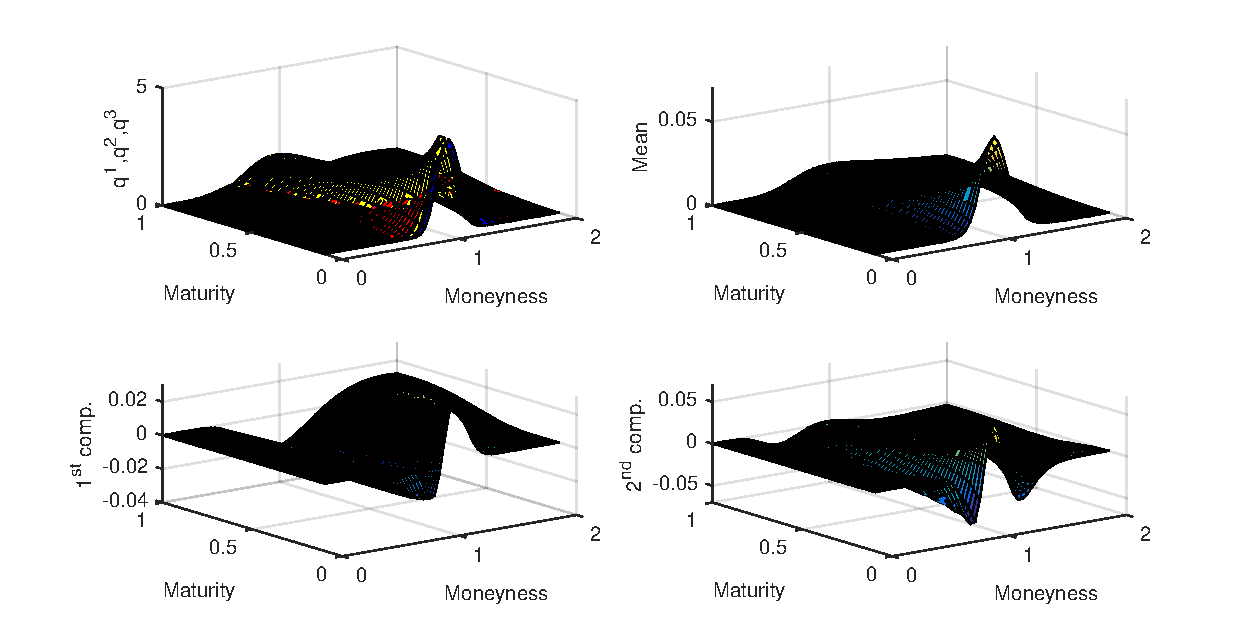
\includegraphics[width=1.00\textwidth]{Figures/Simulation2}
%\caption{\label{sim1} Simulated mixture components - log-normal densities $q^1$ - red; $q^2$ - blue; $q^3$ - yellow; Mean curve and orthonormal components}
%\end{center}
%\end{figure}


Without loss of generality, we set $r_{i\tau}=0$, for each day $i=i,\ldots,N$. %Then, in terms of the notations of section \ref{t2}, $X_i(m,\tau)=C_i(m,\tau)$ and $X_i^{(d)}(m,\tau)=q_i(m,\tau)$, for $d=(2,0)$. 
%The loadings are simulated from the positive half-standard normal distribution, then standardized to sum up to one. 
%Remember tat $r_{s,i}=\frac{s_i}{s_0}$. The stock price follows a geometric Brownian motion  with $\log(s_{i} / s_{i-1})\sim \mathbb{N}(0.03,0.18)$ for ordered time points $i=1,\ldots N$. The parameter choice corresponds to the empirical mean and variance of the stock index log-returns in the real data study. The starting value is $s_{0}=100$ and we fix the risk free rate to $0.02$ p.a. for all days. 
We construct a random grid for each observed curve $X_i$ by simulating points $t_{ik}=(m_{ik},\tau_{ik}), \; k=1,\dots,T$ from a uniform distribution with continuous support $[0.5,1.8]\times[0.2,0.7]$. %The first dimension is moneyness and the second maturity to match the features in the real data, see next subsection. 
%To get a coverage of the entire space like in the case of real data when few observations in the maturity direction are present 
%We additionally require that for ordered $\tau_l$, $\EE\left[\tau_l-\tau_{l+1}\right] = \frac{1}{3}$. 
Finally, we record noisy discrete observations of the call functions with the additive error term i.i.d. $\varepsilon_{ik} \sim \operatorname{N}(0,0.1^2)$.%, with $\sigma_{\varepsilon}=0.02$. 

%1. we know the shape of the orthogonal components 
%2. identification depends on the covariance of the loadings - in our example only two are identified - it depends on the sample covariance, depending on the signal to error ratio - can be viewed as error??? 
%3. implied volatility variation 
%By construction using a mixture of $L$ factors and $\sum_{l=1}^{L+1} w_{il}=1$ this model has $L-1$ principal components. 
%The simulated components $q_l$ and their orthogonal counterparts are shown in figure \ref{?}. 

%However, in our example, the third component is theoretically not identifiable. they are not always identifiable from the observations $q$ (or noisy versions of them). 


%The simulated components $q$ and their orthogonal counterparts are shown in figure \ref{?}. In our example $Var(w_1)=Var(w_2)=Var(w_3)=33\%$, while the variance of the orthogonal components are $97.97\%$, $1.77\%$ and $0.26\%$ respectively.

The true SPDs given by equation (\ref{trueSPD}) are used to verify the performance of $\hat{X}^{(d)}_{FPCA_1},\;  \hat{X}^{(d)}_{FPCA_2}$ and of the individually estimated curves $\hat{X}^{(d)}_{Indiv.}$, in terms of mean integrated squared error (MSE), i.e., $T^{-1} \sum_{k=1}^T \left\{X^{(d)}(t_{ik}) - \hat{X}^{(d)}_\bullet (t_{ik})\right\}^2$, for $d=(2,0)$. For evaluation we generate a common grid of 256 points from a uniform distribution.
%the mean squared error (MSE), which averages the errors for each curve  over number of curves time observations per curve. a discrete version of N^{-1} \sum_{i=1}^N 
To derive the optimal bandwidth in each case we stick to the rule-of-thumb approach presented in Section \ref{implementation}. %We adjust the rule to the given circumstance. 
The bandwidth for the individually smoothed curve $i$ is derived by replacing $\hat{p}^{(\nu)}_{ir}$ in (\ref{rulethumb}) by one and zero otherwise.
The performance is recorded for sample sizes $N$ of $10$ and $25$ with $T$ observations per day of size $50$ and $250$.  This procedure is repeated 500 times to get reliable results, mean, variance and the inter quartile distance based at the MSE of the repetitions are given in Table \ref{fig:SimuResults}. %to show how fast the asymptotics take effect
%To show that our bandwidth criteria works, we have experimented with 100 curves. We repeated the procedure 1000 times to show how fast the asymptotics take effect. 

 %In particular, for $b$ we have experimented with various bandwidths, e.g. we looked at the mean, minimum and maximum of individually optimal bandwidths. The best results are obtained for the maximum, hence, we report only these results in the following.
%Goodness of fit is measured in terms of the mean square error (MSE) per curve. We average the results for each repetition and report the sample performance using the average mean square error (AMSE). 
%Their effects are evaluated in the following simulation studies.
%We considered various simulation scenarios based on the combinations of the case of errors size and number of observation points and curves. 
%Tables \ref{table1} through \ref{table3} summarize the simulation results. %estimation results for curves estimated by FPCA and simple smoothing respectively. %For computing we use empirical centered true values. To guarantee a fair comparison we display AMSE for individual 


%smoothed curves as well with the optimal bandwidth for individual curves and in addition for the same level of smoothing like the FPCA (marked by *). %With a single exception FPCA performs better than its benchmark model. %The distribution of AMSE is synthetized in the boxlots from figure (\ref{boxplots}).
%We need to report how the optimal constant changes with the size of the noise. If there are differences then we'll get the constant equal to the our estimated $\sigma_{\varepsilon}$ in the real data example. 
%The results for the one repetition is summarized here: we find two factors because the third one is a linear function of the two. Make plot + ....
\begin{table}
\footnotesize
  \centering
  \begin{tabular}{c|c|c|c|c|c|c|c|c|c}
    \hline
    \hline
    &$T$&\multicolumn{4}{c|}{50}&\multicolumn{4}{c}{250}\\
    %\cline{3-6} 
		\hline
    $N$&$\hat{X}^{(d)}_\bullet$&Mean&Var&Med&IQR&Mean&Var&Med&IQR\\
    \hline
    \multirow{3}{12pt}{10}	&\footnotesize $FPCA_1$& 0.1876 & 0.0367 &0.1300 &0.1325& 0.0780 & 0.0025 &0.0643&0.0546\\
													&\footnotesize $FPCA_2$  & 0.2238 & 0.1212 &0.1295 &0.1466& 0.0762 & 0.0026 &0.0630&0.0518\\
													&\footnotesize $Indiv.$  & 0.2709 & 0.0900 &0.1928 &0.1838& 0.1105 & 0.0054 &0.0916&0.0708\\
								\hline
    \multirow{3}{12pt}{25}&\footnotesize $FPCA_1$& 0.0917 & 0.0066 &0.0680&0.0580& 0.0404&0.0006 & 0.0336 &0.0223\\
													&\footnotesize $FPCA_2$& 0.1553 & 0.0966 &0.0878&0.0887& 0.0586&0.0016 & 0.0489 &0.0406\\
													&\footnotesize $Indiv.$& 0.2691 & 0.0995 &0.1889&0.1848& 0.1111&0.0052 & 0.0916 &0.0719\\
    \hline  \hline
  \end{tabular}
  \caption{Results of the simulation described in Section \ref{simstudy} with different values for $T$ and $N$. $FPCA_1$ and $FPCA_2$ are superior in sense of MSE over the individual estimation of the derivatives in each setting. $FPCA_1$ is better than $FPCA_2$ except for $N=10$, $T=250$. For $FPCA_1$ and $FPCA_2$ the estimation improves with raising $N$ and $T$. These results support our asymptotic results given by Proposition \ref{Mbias} and \ref{curvebias}. }
  \label{fig:SimuResults}
\end{table}


%
%\begin{center}
%\textbf{[Insert Table~\ref{table1} approximately here.]} 
%\end{center}
%\begin{center}
%\textbf{[Insert Table~\ref{table2} approximately here.]} 
%\end{center}
%\begin{center}
%\textbf{[Insert Table~\ref{table3} approximately here.]} 
%\end{center}

Both FPCA based approaches gives better estimates for the derivative of the call functions than an individually applied local polynomial estimator of the individual curves. Both the mean and the median of the MSE are smaller which is a result of the additional average over $N$ for the basis functions as given by Proposition \ref{curvebias}. However, the $FPCA_1$ method performs decisively better for small $T$ than the other two both in terms of mean and standard deviation of the mean squared error. 
In addition  $FPCA_1$ benefits more from raising $N$ then $FPCA_2$. With small $T$ for $FPCA_2$ and individual smoothing the variability of MSE is much bigger than for $FPCA_1$ while the median of $FPCA_1$ and $FPCA_2$ are comparable. This means individual smoothing and $FPCA_2$  must behave much worse than $FPCA_1$ in some instances while $FPCA_1$ was able to stabilize the estimates. To get the same effect using $FPCA_2$ a much bigger $T$ is needed. A possible explanation for this behavior is given by Proposition \ref{Mbias}. The rates of convergence to estimate elements of the dual matrix solely rely on $T$ thus it is nearby that facing small $T$ some of the thereby derived loadings are inaccurate.
%For all estimation procedures the interquartile range (IQR) together with the standard deviation suggests that the distribution of MSE has fatter tails than normal and the comparison of mean and median also suggests a non normal distribution. %, in particular for the direct method. 

%Its performance depends on the sample characteristics and using it in applications has an associated higher risk. 
%In addition, the slow improvement in the direct method confirm that the order of convergence is dominated by the fixed number of observations per curve $T$. %the sample size of curves shall be very large to give comparable convergence with the indirect method. \color{red}Also possible that it never does, we need to increase the observation points. (Unless we increase the observation points ... it will never be asymptotically equivalent???) \color{black}


%Contrasting the interquartile range (IQR) with the standard deviation suggests that the distribution of MSE has fatter tails than normal, in particular for the direct method. 

%In particular, the direct method has many Looking at the IQR suggests that the large variance is due to the very bad performance of FPCA_2 in some of the cases (not necessarily outliers). The standard deviation stabilizes when we increase the number of curves (or not?). the small improvement in the fpca2 suggests that the number of curves shall be much higher. 

